% Digital Logic Report Template
% Created: 2020-01-10, John Miller

%==========================================================
%=========== Document Setup  ==============================

% Formatting defined by class file
\documentclass[11pt]{article}

% ---- Document formatting ----
\usepackage[margin=1in]{geometry}	% Narrower margins
\usepackage{booktabs}				% Nice formatting of tables
\usepackage{graphicx}				% Ability to include graphics
\usepackage[section]{placeins}      % Stops floats from happening

%\setlength\parindent{0pt}	% Do not indent first line of paragraphs 
\usepackage[parfill]{parskip}		% Line space b/w paragraphs
%	parfill option prevents last line of pgrph from being fully justified

% Parskip package adds too much space around titles, fix with this
\RequirePackage{titlesec}
\titlespacing\section{0pt}{8pt plus 4pt minus 2pt}{3pt plus 2pt minus 2pt}
\titlespacing\subsection{0pt}{4pt plus 4pt minus 2pt}{-2pt plus 2pt minus 2pt}
\titlespacing\subsubsection{0pt}{2pt plus 4pt minus 2pt}{-6pt plus 2pt minus 2pt}

% ---- Hyperlinks ----
\usepackage[colorlinks=true,urlcolor=blue]{hyperref}	% For URL's. Automatically links internal references.

% ---- Code listings ----
\usepackage{listings} 					% Nice code layout and inclusion
\usepackage[usenames,dvipsnames]{xcolor}	% Colors (needs to be defined before using colors)

% Define custom colors for listings
\definecolor{listinggray}{gray}{0.98}		% Listings background color
\definecolor{rulegray}{gray}{0.7}			% Listings rule/frame color

% Style for Verilog
\lstdefinestyle{Verilog}{
	language=Verilog,					% Verilog
	backgroundcolor=\color{listinggray},	% light gray background
	rulecolor=\color{blue}, 			% blue frame lines
	frame=tb,							% lines above & below
	linewidth=\columnwidth, 			% set line width
	basicstyle=\small\ttfamily,	% basic font style that is used for the code	
	breaklines=true, 					% allow breaking across columns/pages
	tabsize=3,							% set tab size
	commentstyle=\color{gray},	% comments in italic 
	stringstyle=\upshape,				% strings are printed in normal font
	showspaces=false,					% don't underscore spaces
}

% How to use: \Verilog[listing_options]{file}
\newcommand{\Verilog}[2][]{%
	\lstinputlisting[style=Verilog,#1]{#2}
}




%======================================================
%=========== Body  ====================================
\begin{document}

\title{ELC 2137 Lab 10: 7-segment Display with Time-Division Multiplexing}
\author{Maddie Vorhies}

\maketitle

\section*{Summary}

The goal of this lab was to use lab 8 and lab 9 and put them together to create a 7-segment display with time- division multiplexing. In order to do this, I needed the top9 module from lab 9 and I needed the sseg4 from lab 8. In addition to it, I also created a counter and a show2c. The counter has a timer that is used to get a short pulse when the counter reaches its maximum value. The show2c is used to output the 2's compliment of the incoming number. To check the counter and the show2c, I created a testbench. Once the testbench was successfully executed, I was able to combine the top9 from lab 9, the sseg4 from lab 8, and the counter and show2c from lab 10 to create a mini calculator. The calculator is able to add and subtract. If needed, it will display a negative number on the board. I tested my board to make sure that it worked and I was successfully able to output both a positive and a negative number.  


\section*{Results}

\begin{figure}[ht]\centering
	\caption{Simulation Waveform for counter (N = 4)}
	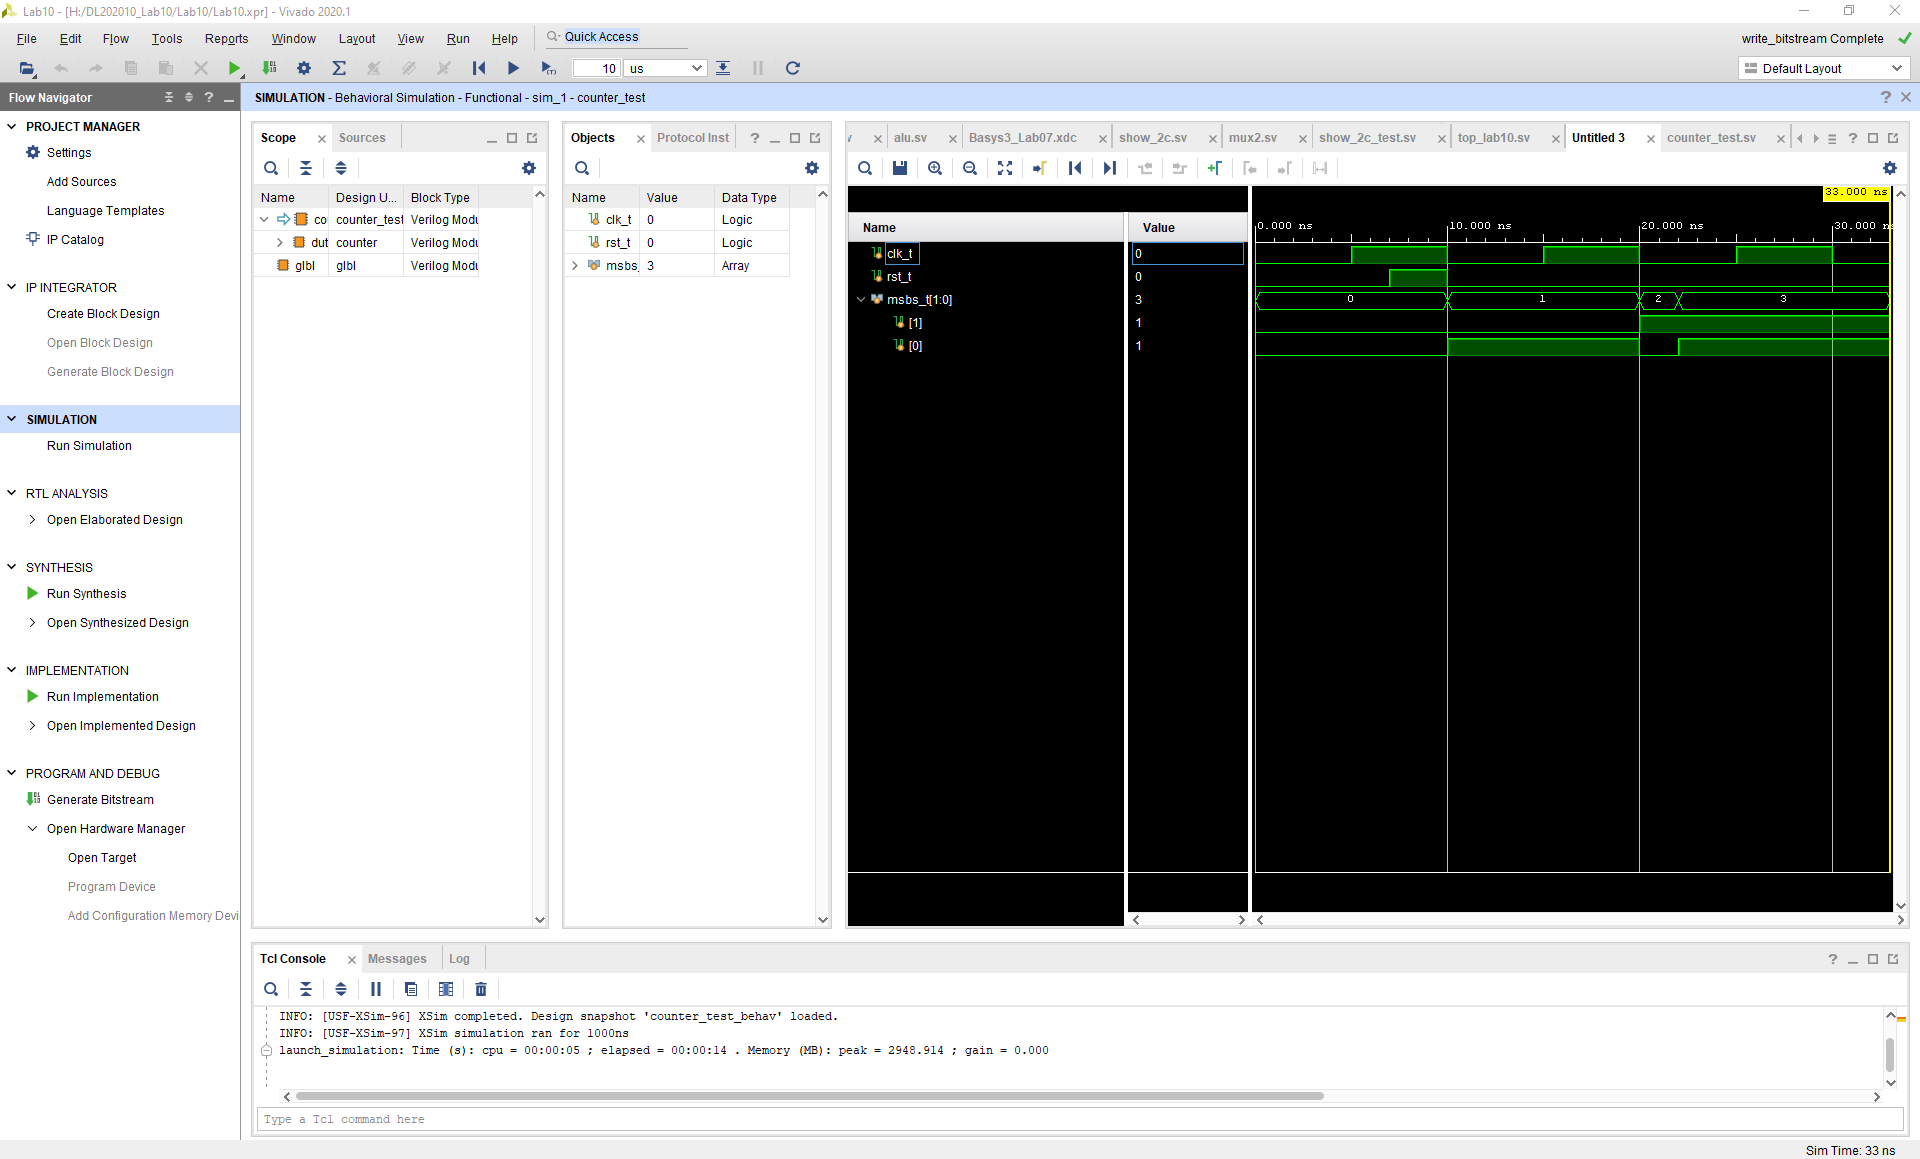
\includegraphics [width=1\textwidth,trim=640 550 10 135, clip]{counter_sim}
\end{figure}

\begin{figure}[ht]\centering
	\caption{Simulation Waveform for show2c}
	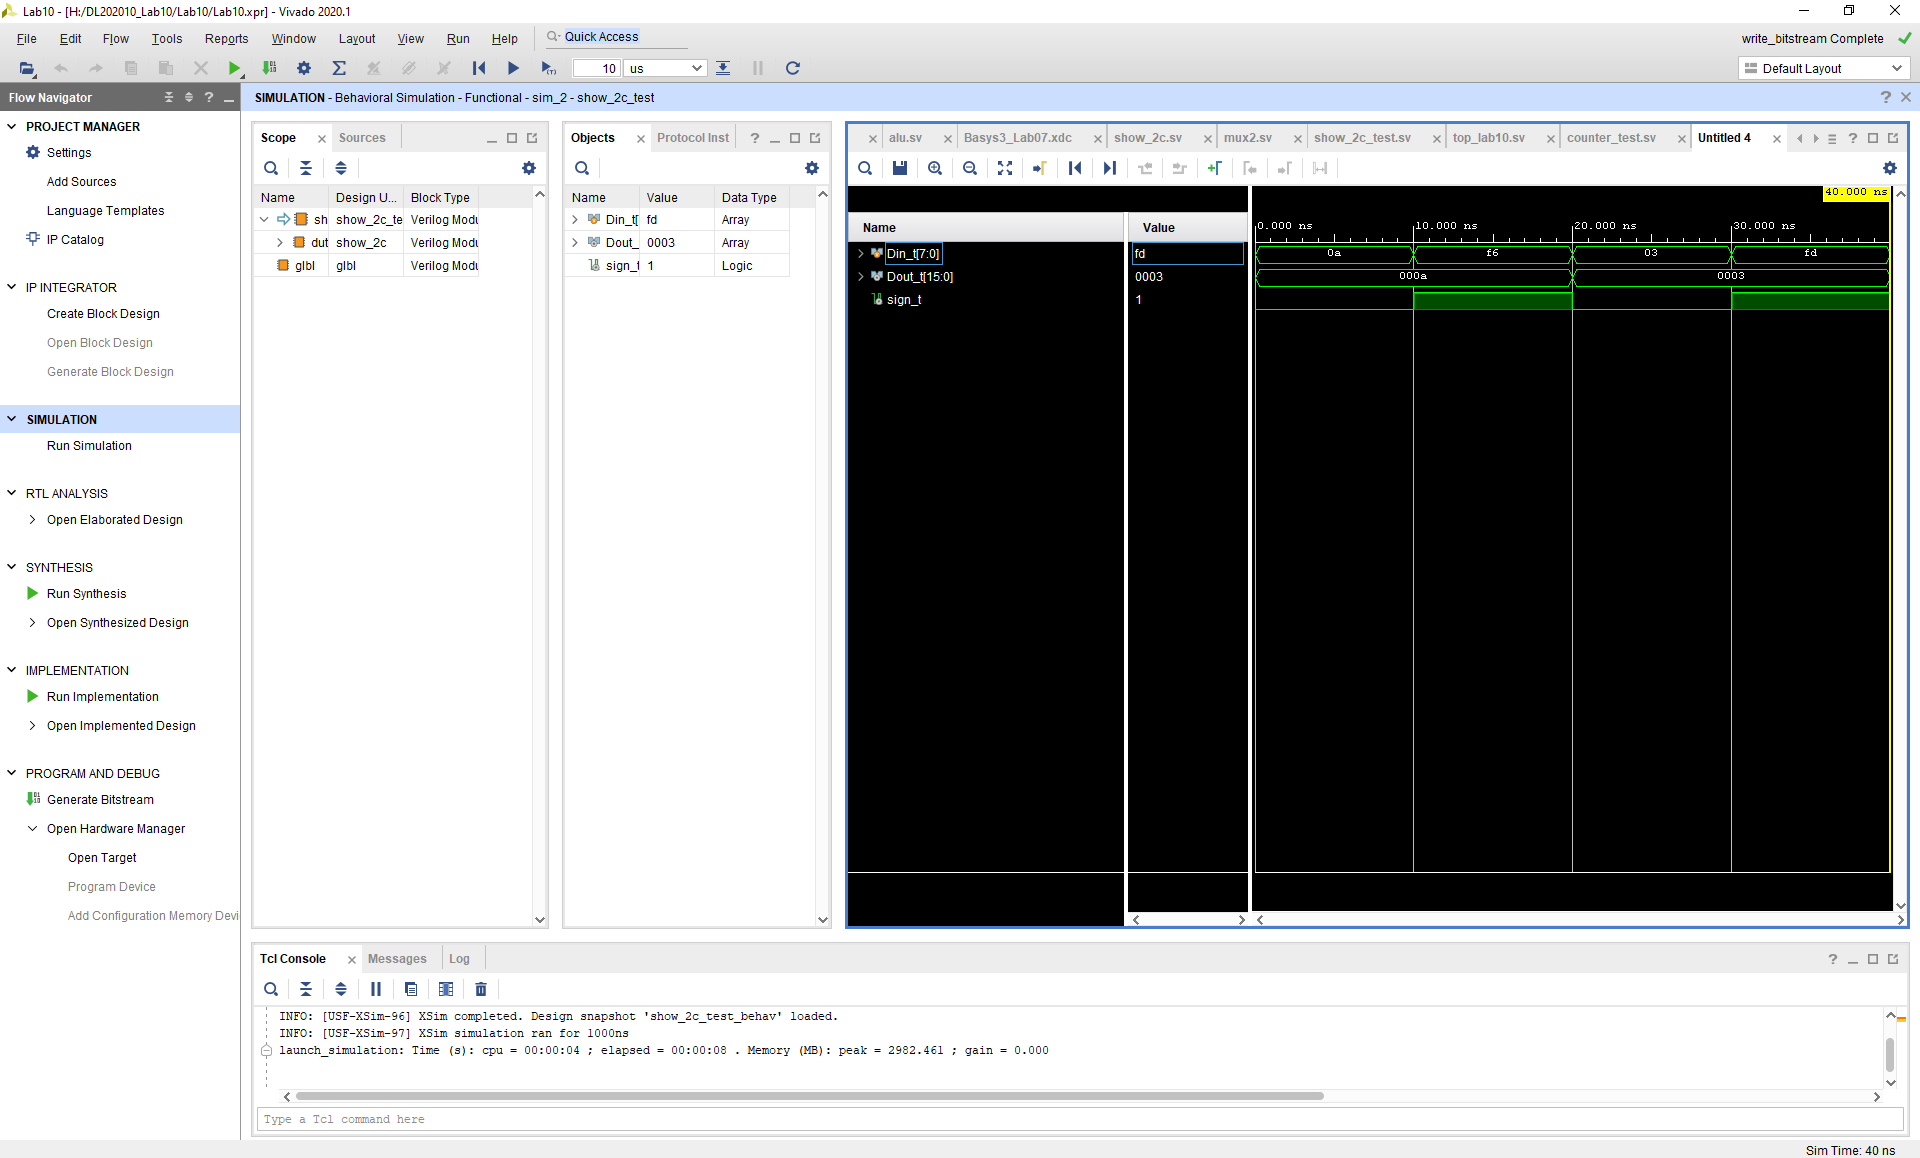
\includegraphics [width=1\textwidth,trim=640 550 10 135, clip]{show_2c_sim}
\end{figure}

\begin{figure}[ht]\centering
	\caption{4-digits at full strength and no blinking (N = 20)}
	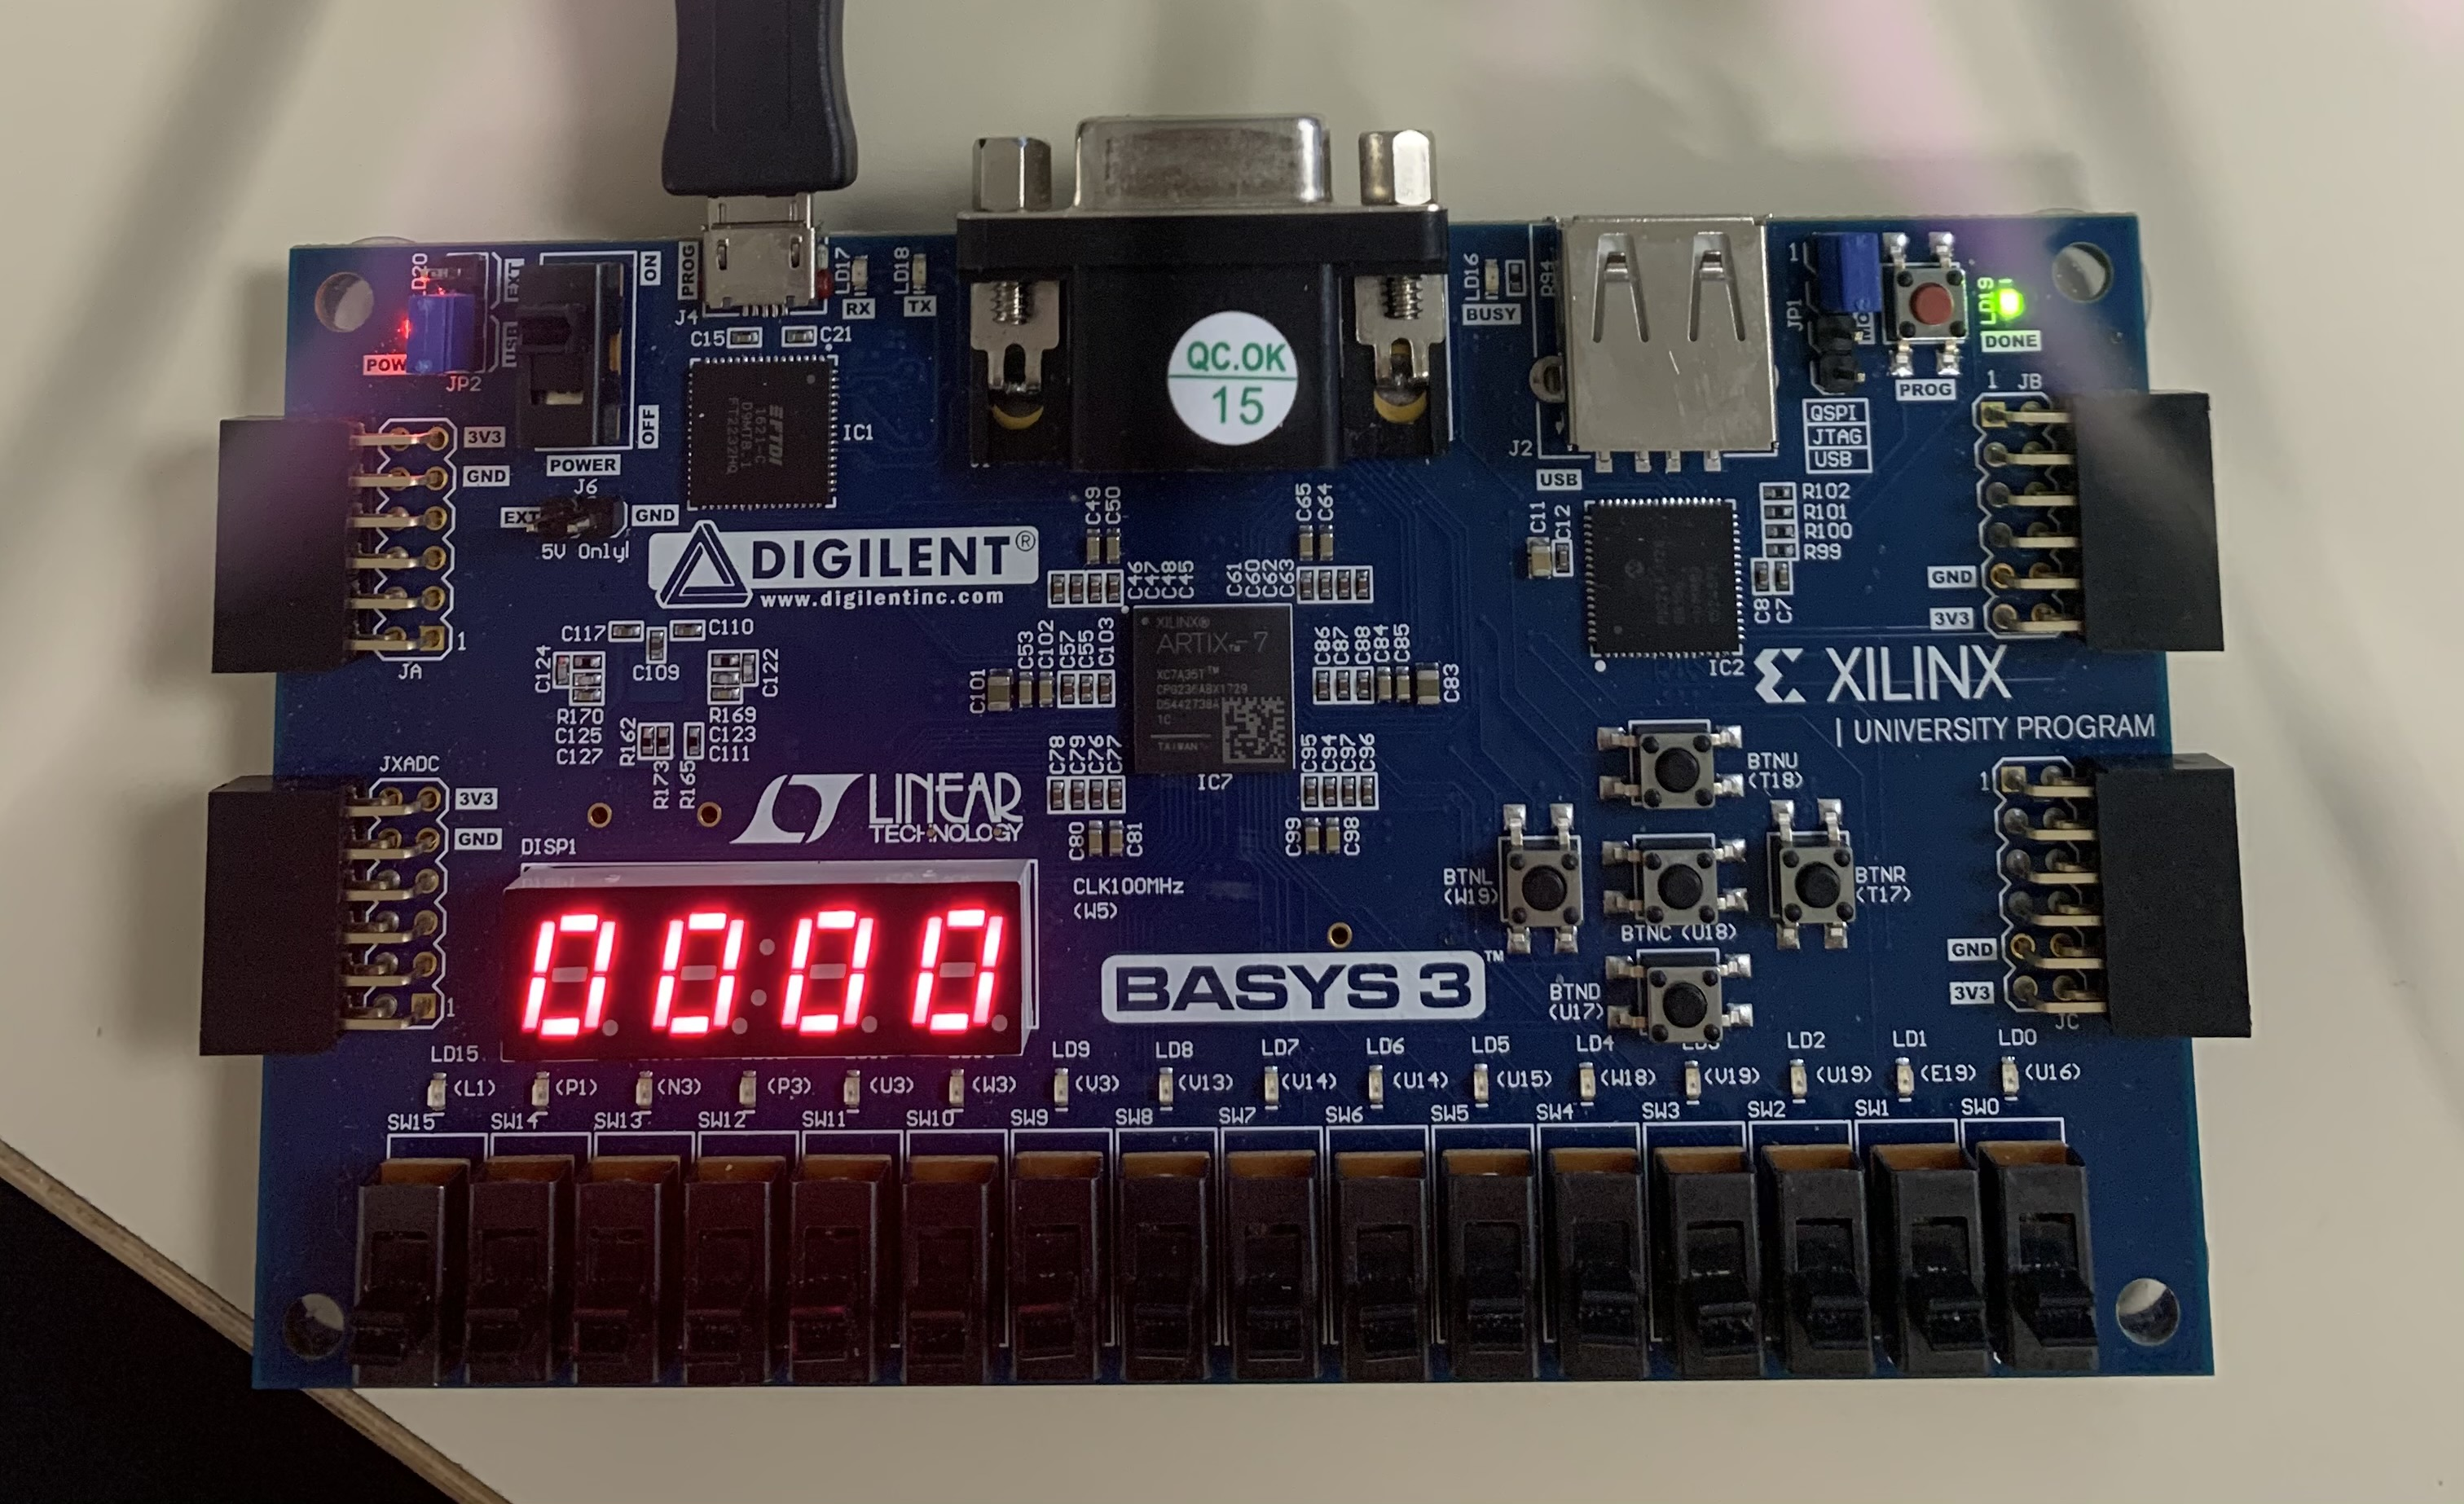
\includegraphics [width=0.75\textwidth,trim=0 0 0 0, clip]{pic1}
\end{figure}

\begin{table}[h]\centering
	\begin{tabular}{cc}
		Positive number & Negative Number \\
		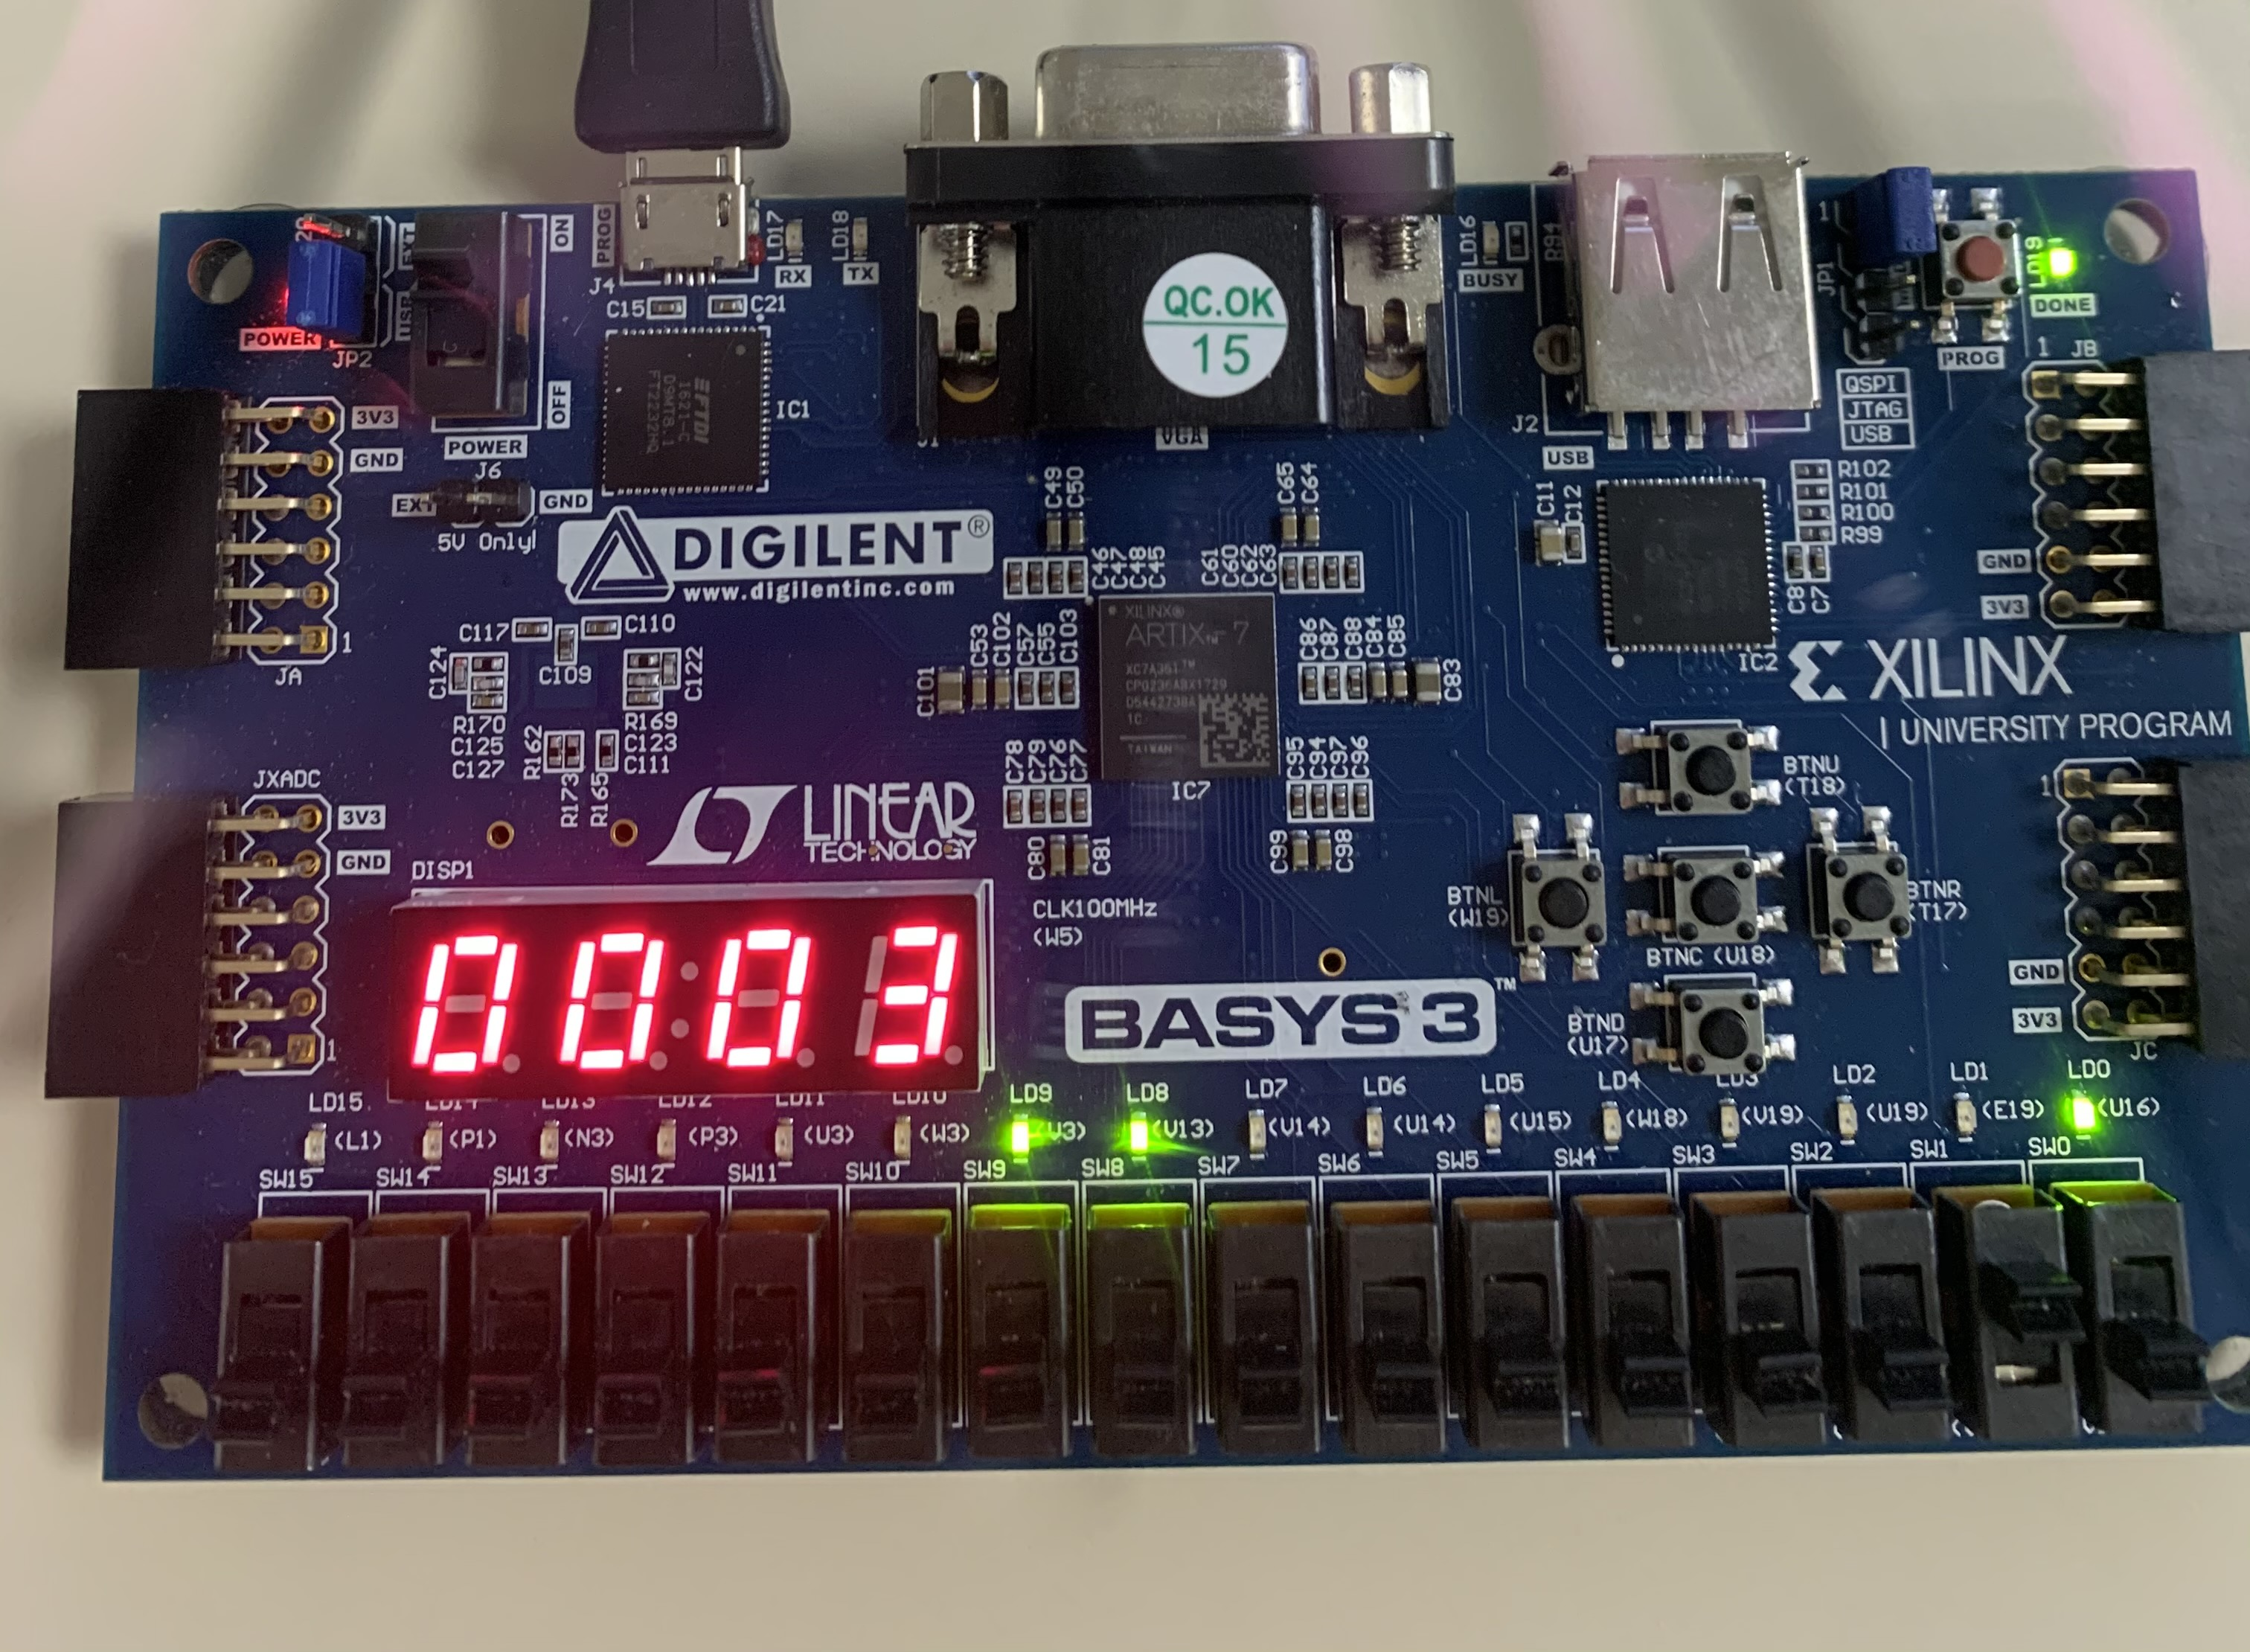
\includegraphics [width=0.5\textwidth,trim=0 0 0 0, clip]{pic2} &
		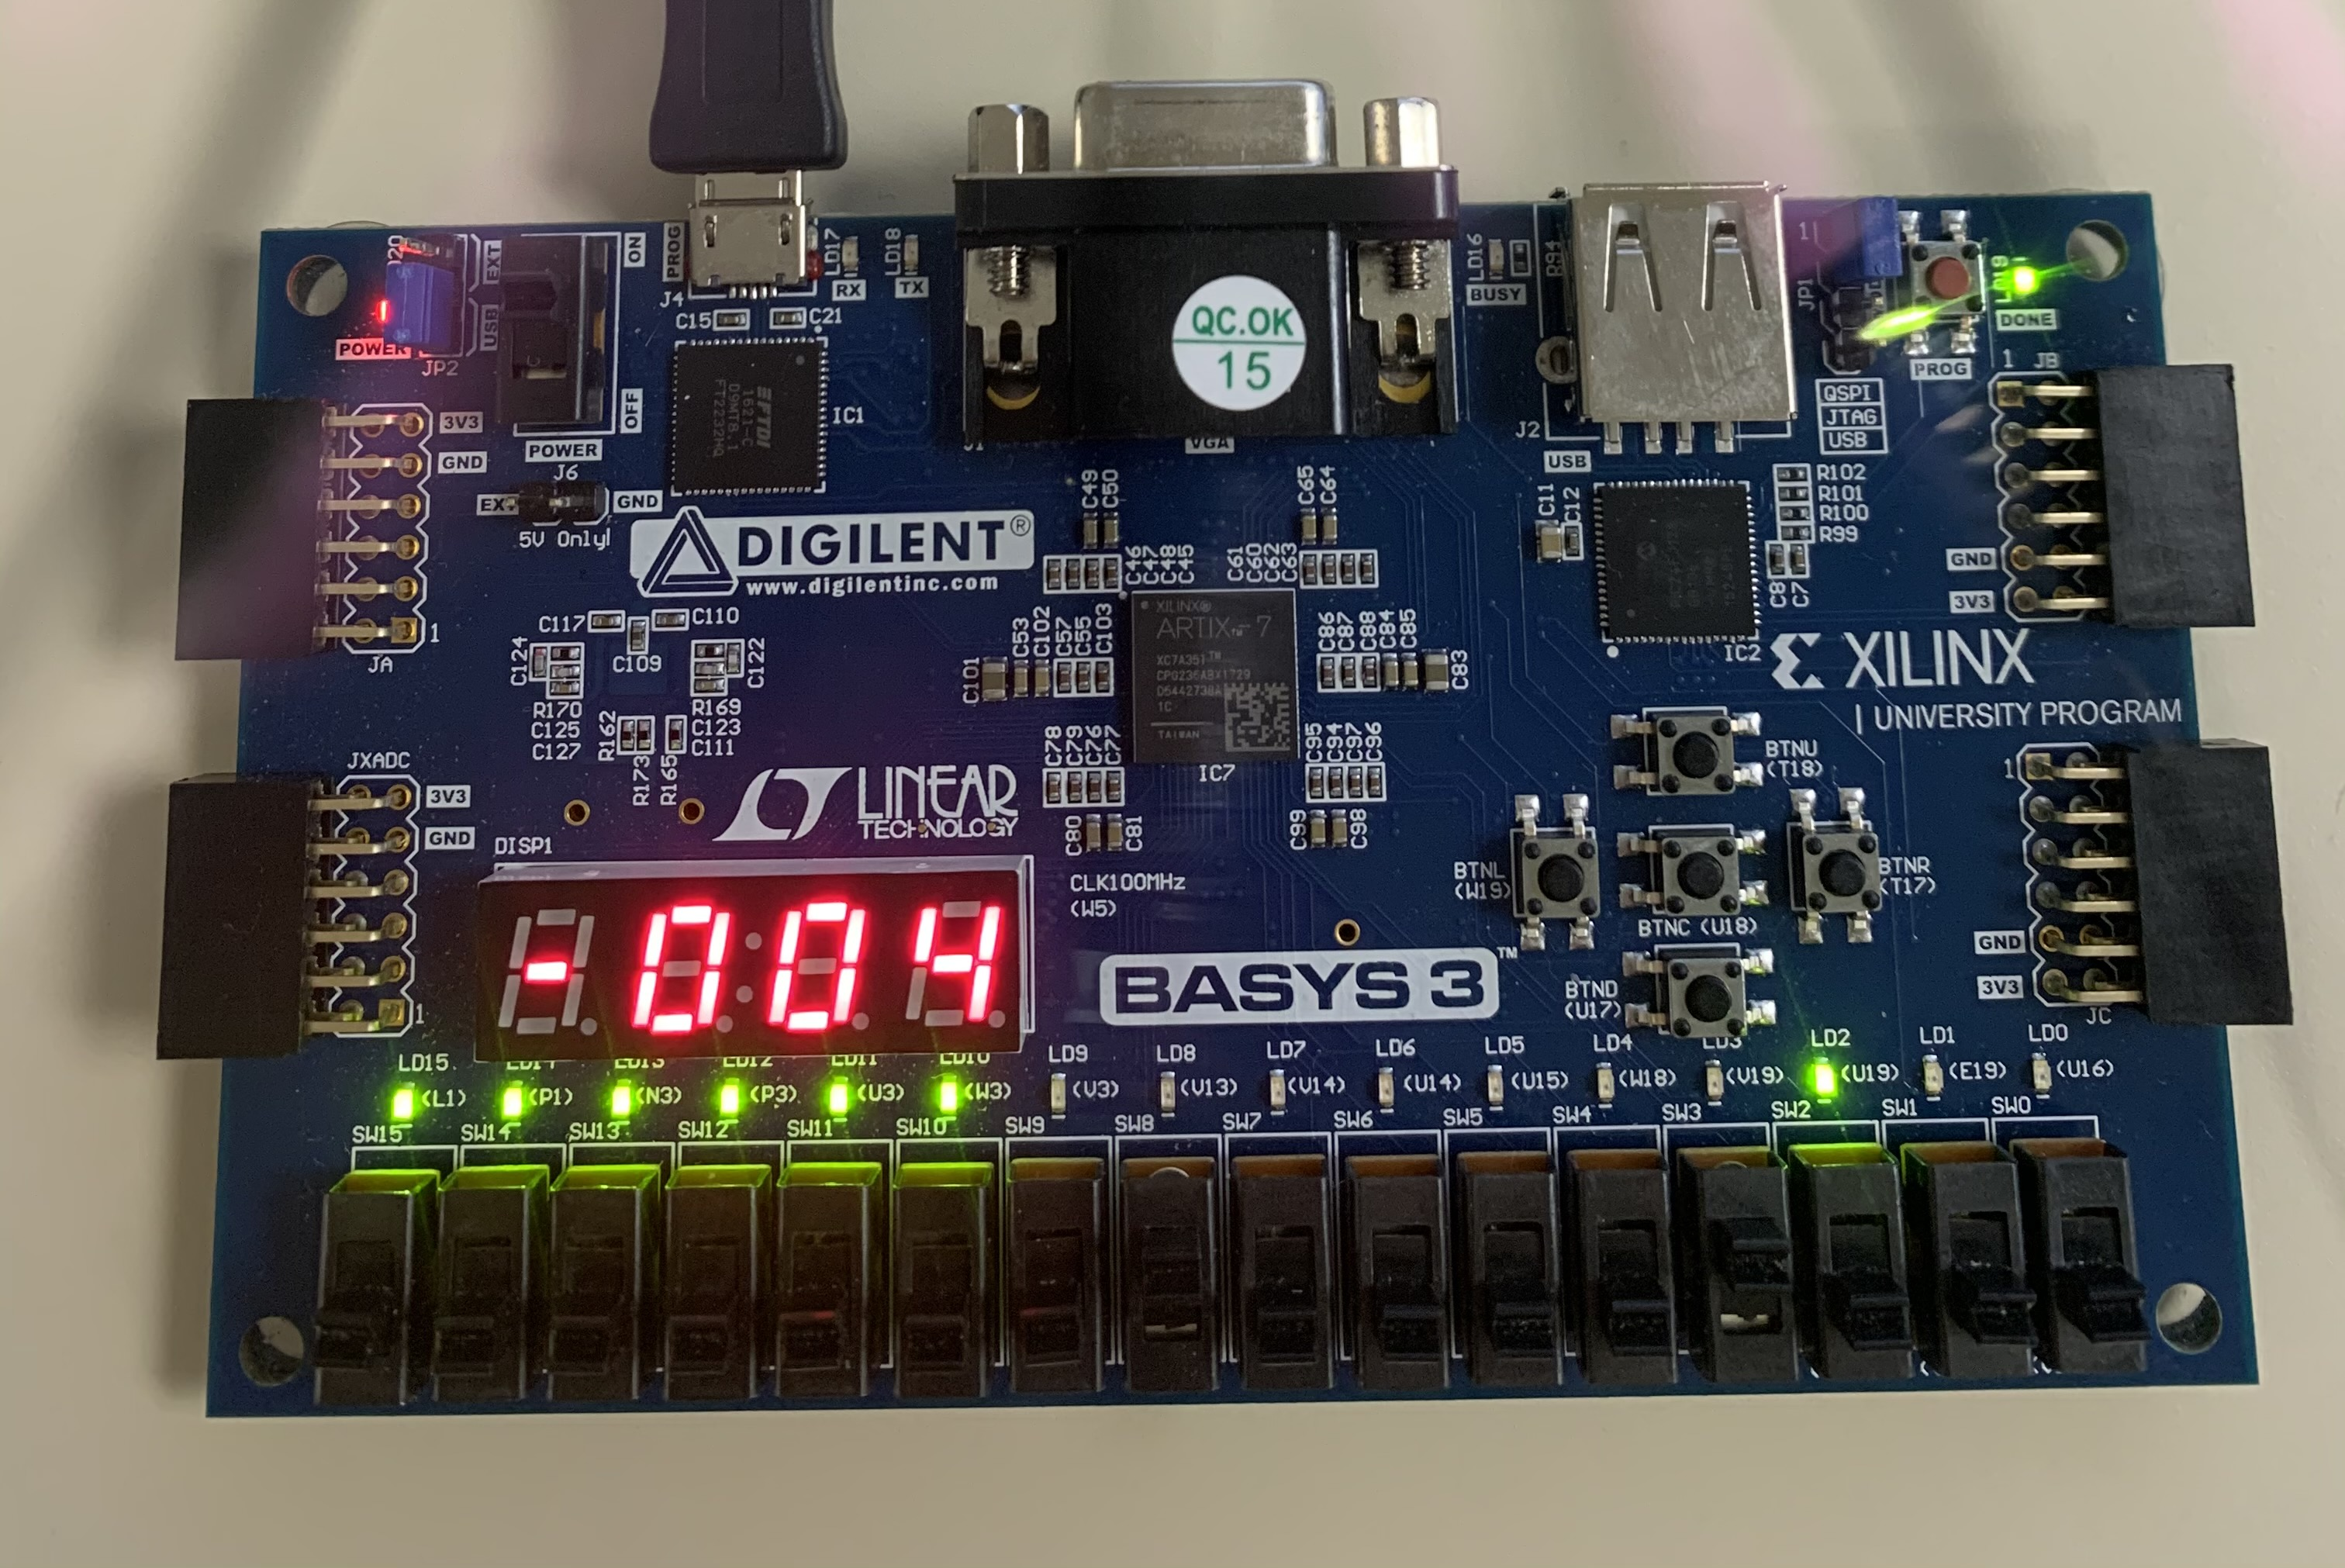
\includegraphics [width=0.55\textwidth,trim=0 0 0 0, clip]{pic3} \\
	\end{tabular}
	\caption{Board Pictures}
	\label{fig:sim_with_table}
\end{table}



\section*{Code}

\Verilog{Lab10/systemverilog/counter.sv}

\Verilog{Lab10/systemverilog/counter_test.sv}

\Verilog{Lab10/systemverilog/show_2c.sv}

\Verilog{Lab10/systemverilog/show_2c_test.sv}

\Verilog{Lab10/systemverilog/wrapper.sv}

\Verilog{Lab10/systemverilog/top_lab10.sv}


\end{document}
